%\subsection{Neocortical Layer 4/5 Pyramidal Cell Test Suite}
\subsubsection{2a}

%Direct Quote: "widening of the spike shape, decrease of the firing rate and change in the interspike interval distribution". %All these single unit waveform shapes increased their width with temperature.\cite{goldin2017temperature}



%\subsubsection{%\subsection{Section 2.1}
%
%
\subsubsection{Performance of Layer 5 Pyramidal Neuron Somatosensory on NeuronUnit tests of model data agreement}
Hind-limb
\cite{van2016bluepyopt}
To understand the validity of model re-purposing, we tested a model constrained on Layer 5 Somatosensory cortex Pyramidal neurons. A suite of neuronunit tests containing the tests: rheobase value, membrane voltage time constant ($tau_{m})$, input resistance was computed. This multi-compartment, conductance based model served as a useful benchmark, for us to evaluate the relative performance of reduced model fits. originating from the blue brain project \cite{markram2015reconstruction}



% somatosensory cortex, or cell from the l5 somatosensory rat, hind leg region, so it is probably not comparable to NeuroElectro Data.

Significant development work went into making the model eligible to take NeuronUnit tests, to make this complicated conductance based multi-compartment model interoperable with the neuronunit test judging paradigm. The intention is that by making this model inter-operable with NeuronUnit the model will be able to amenable to different, optimization.

This elaborate biophysical model includes the backpropogating dendritic action potential.
%\url{}



\begin{figure}
\begin{center}


\centering
\begin{subfigure}{.2\textwidth}
  \centering
    %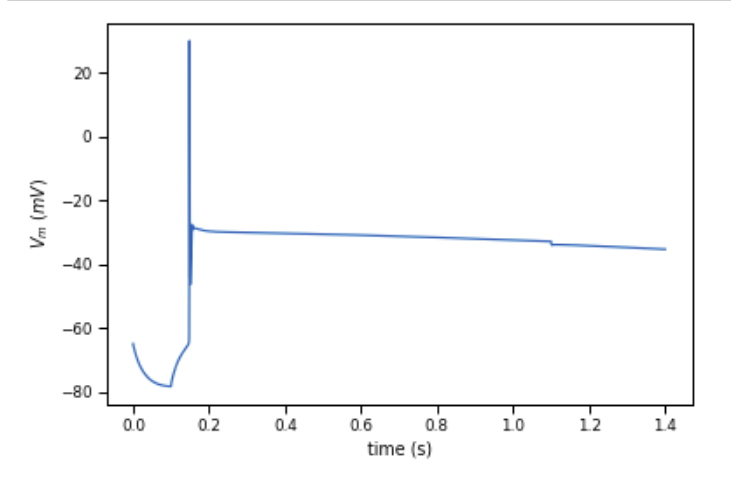
\includegraphics[scale=0.5]{figures/correct_active_l5pc.png}
    \caption{A current injection sufficient for causing a single spike is applied for a whole second from $100ms-1100ms$}
  \label{fig:sub1}
\end{subfigure}

As a reference point for understanding 
    \caption{The spike shape is very brief in duration, and so it is worth zooming in for a closer look}

\centering
\begin{subfigure}{.2\textwidth}
  \centering
    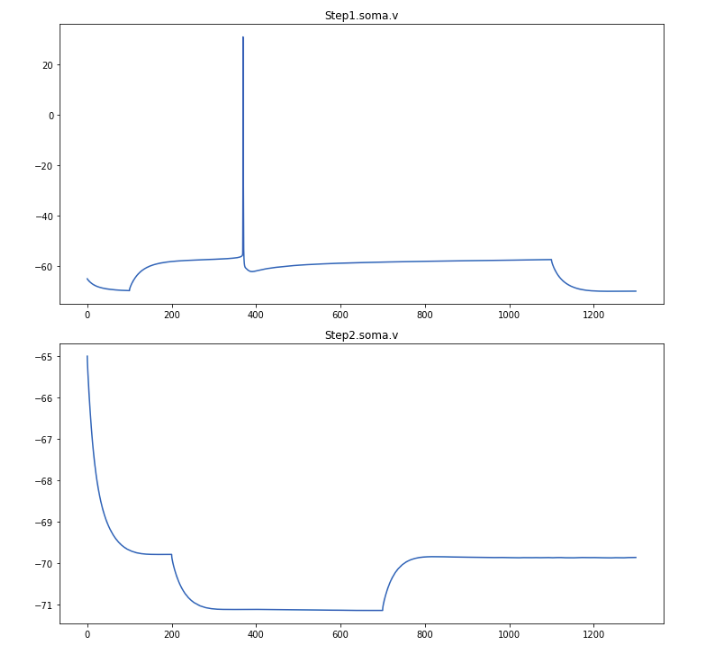
\includegraphics[scale=0.5]{figures/L5Somatosensory_not_optimized.png}
    \caption{$V_{m}$ in $(mV)$ versus time $ms$, plots include a suprathreshold (top) and subthreshold stimulus (below)}
  \label{fig:brief_shape}
\end{subfigure}

\centering
\begin{subfigure}{.2\textwidth}
  \centering
    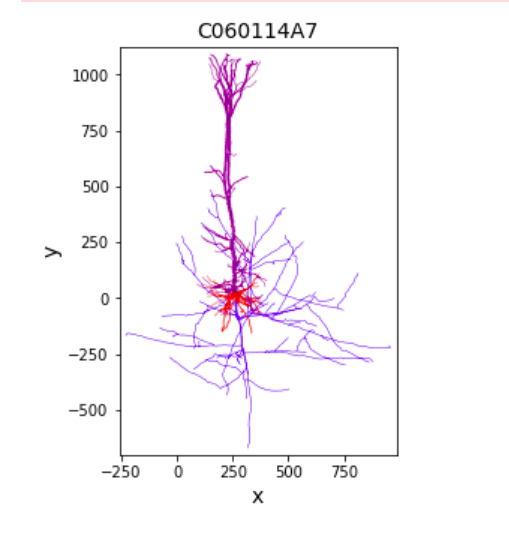
\includegraphics[scale=0.5]{figures/morphology_view.png}
    \caption{This multi-compartment model is spatially extended, so a 2D depiction of its 3D form is warranted.}
  \label{fig:brief_shape}
\end{subfigure}

\begin{subfigure}{.2\textwidth}
  \centering
    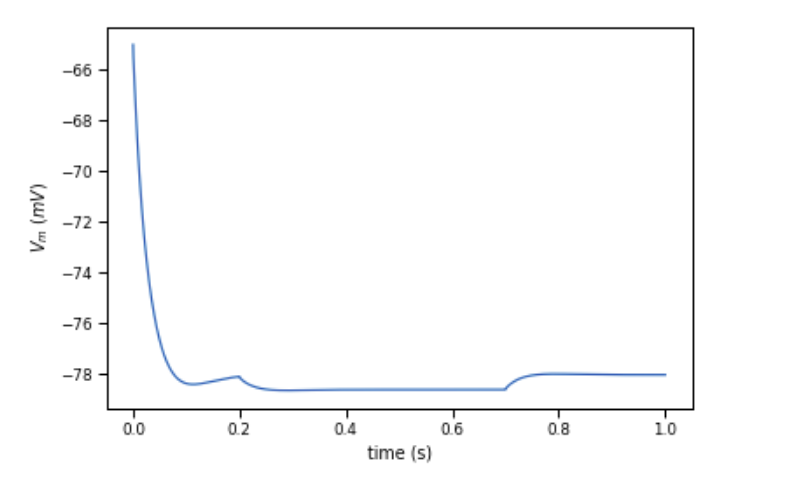
\includegraphics[scale=0.5]{figures/correct_passive_l5pc.png}
    \caption{A current injection value of -$10pA$ is applied to the cell for the duration of $200ms-700ms$}
  \label{fig:passive_properties_fine}
\end{subfigure}
\label{fig:test}
\end{center}
\end{figure}


\subsubsection{Optimized Results}
\begin{table}[ht]
\centering
\resizebox{\textwidth}{!}{
\begin{tabular}{lllll}
\toprule
{} & observations &                 predictions &   Z-Scores \\
\midrule
RheobaseTest                   &    213.85 pA &                   213.85 pA &  2.444e-06 \\
InputResistanceTest            &  120.67 Mohm &  183.56713371523054 megaohm &     0.8102 \\
TimeConstantTest               &     15.73 ms &   0.00016898141845179352 ms &     -2.152 \\
CapacitanceTest                &    150.58 pF &    0.0009205428827686333 pF &     -1.078 \\
RestingPotentialTest           &    -68.25 mV &        -71.8621793344104 mV &    -0.5533 \\
InjectedCurrentAPWidthTest     &      1.21 ms &                    2.075 ms &      1.623 \\
InjectedCurrentAPAmplitudeTest &     80.44 mV &        63.31628969975701 mV &     -1.343 \\
InjectedCurrentAPThresholdTest &    -42.74 mV &      -44.863238963316746 mV &    -0.2646 \\
\bottomrule
\end{tabular}}
\end{table}

A test suite was constructed using NeuroElectro for the layer 4/5 prefrontal cortex neuron pyramidal cell, and we were able to evaluate this layer 5 PC cells against the criteria of the neuroelectr test suite. Note the unnatural looking brief spike duration of the model cell spike  \ref{fig:brief_shape}. It is possible that the majority neuroelectro experiments on the layer 5 pyramidal cell were conducted under room temperature as opposed to body temperature, as there is evidence that the temperature of cortical tissue modulates spike width \cite{goldin2017temperature}, in particular cooling can contract their spike width

%%
% https://neuroelectro.org/data_table/36261/
%%
% from spike width table: 0.65 ± 0.13	1.04 ± 0.25**	0.51 ± 0.03**	0.59 ± 0.06	0.61 ± 0.03
%%
%

Due to computational limitations this model was only run for 
$12$ offspring, and $30$ generation. Actually a minimum of $MU=100$, $NGEN =100$ was prescribed by the scientists who optimized the initial model, however such a large compute job required prohibitive computational resources.


The unoptimized model had statistics:
$(\chi^{2},p_{value})=(13.5609360364, 0.093951963105254)$

The optimized model produced statistics
$(\chi^{2},p_{value})=(6.632440090005973 0.5767576828862497)$

Optimization then clearly improves the model, however, it does not bring the model  biological plausibity.





This can be improved by omitting some of the worst tests, overall, the tests are compromized.



It is worth noting that the layer 5 neocortical pyramidal neuron was very slow to dispatch relative to the reduced models developed in this thesis work. Where as a typical reduced model described here evaluated in the order of $~0.0025 seconds$, this model on average took $5.74$, for a single run and $34.8$ to solve for the models Rheobase, current.

This model was pre-optimized to fit to spike times and F/I mainly, and so it should not necassarily be expected to fit other electrical charactersistics of the cell. Only the rheobase test, and the time constant test seemed to fall within the range of biological plausibility.
None the less, this model remains a useful benchmark for reduced neuronal models.